%%%%%%%%%%%%%%%%%%%%%%%%%%%%%%%%%%%%%%%%%%%%%%%%%%%%%%%%%%%%%%%%%%%%%%
% Overleaf (WriteLaTeX) Example: Molecular Chemistry Presentation
%
% Source: http://www.overleaf.com
%
% In these slides we show how Overleaf can be used with standard 
% chemistry packages to easily create professional presentations.
% 
% Feel free to distribute this example, but please keep the referral
% to overleaf.com
% 
%%%%%%%%%%%%%%%%%%%%%%%%%%%%%%%%%%%%%%%%%%%%%%%%%%%%%%%%%%%%%%%%%%%%%%
% How to use Overleaf: 
%
% You edit the source code here on the left, and the preview on the
% right shows you the result within a few seconds.
%
% Bookmark this page and share the URL with your co-authors. They can
% edit at the same time!
%
% You can upload figures, bibliographies, custom classes and
% styles using the files menu.
%
% If you're new to LaTeX, the wikibook is a great place to start:
% http://en.wikibooks.org/wiki/LaTeX
%
%%%%%%%%%%%%%%%%%%%%%%%%%%%%%%%%%%%%%%%%%%%%%%%%%%%%%%%%%%%%%%%%%%%%%%

\documentclass[xcolor=dvipsnames]{beamer}

\usetheme{Madrid}
\useoutertheme{split} % Alternatively: miniframes, infolines, split
\useinnertheme{circles}

%%%%%%%%%%
% Giorgio Morandi #colors_1
\definecolor{color0}{HTML}{372639}
\definecolor{color1}{HTML}{C2A4C0}
\definecolor{color2}{HTML}{816288}
\definecolor{color3}{HTML}{C6926C}
\definecolor{color4}{HTML}{D5BEA9}
\definecolor{color5}{HTML}{DBCAD3}
%%%%%%%%%%

%%%%%%%%%%
\setbeamercolor{normal text}{bg = color5!25, fg = color0}
%\setbeamercolor{alerted text}{bg = color5, fg = color1}
%\setbeamercolor{example text}{bg = color5, fg = color1!50!color0}

\setbeamercolor{palette primary}{bg = color3, fg = color5!50}
%\setbeamercolor{palette secondary}{bg = color1, fg = color5}
%\setbeamercolor{palette tertiary}{bg = color4, fg = color5}

\setbeamercolor{palette quaternary}{bg = color2!50, fg = color0!75}

\setbeamercolor{structure}{bg = color5!50, fg = color4} % itemize, enumerate, etc

\setbeamercolor{section in toc}{bg = color5!50, fg = color1} % TOC sections

% Override palette coloring with secondary
\setbeamercolor{subsection in head/foot}{bg = color3!50, fg = color2}
% For more themes, color themes and font themes, see:
% http://deic.uab.es/~iblanes/beamer_gallery/index_by_theme.html
%%%%%%%%%%

%%%%%%%%%%
\mode<presentation>
{
  \usetheme{Madrid}       % or try default, Darmstadt, Warsaw, ...
  \usecolortheme{default} % or try albatross, beaver, crane, ...
  \usefonttheme{serif}    % or try default, structurebold, ...
  \setbeamertemplate{navigation symbols}{}
  \setbeamertemplate{caption}[numbered]
} 

\usepackage[english, french]{babel}
\usepackage[utf8x]{inputenc}
\usepackage{chemfig}
\usepackage[version = 3]{mhchem}

% On Overleaf, these lines give you sharper preview images.
% You might want to `comment them out before you export, though.
\usepackage{pgfpages}
\pgfpagesuselayout{resize to}[%
  physical paper width = 8in, physical paper height = 6in]
  
% Here's where the presentation starts, with the info for the title slide
\title[Sujet n°15]{\textsc{Un modèle de coût pour le NoSQL}}
\author{Hao ZHANG}
\institute{\texttt{RECHERCHE COMPARATIVE DU MODÈLE DE COÛT POUR LA NORMALISATION ET LA DÉNORMALISATION DE BD NOSQL }}


\usepackage{datetime}
\newdate{date}{28}{1}{2019}
\date{\displaydate{date}}
%\date{11 novembre 2018}

\logo{\includegraphics[height = 7mm]{images/Logo_ESILV.png}}

\setbeamersize{text margin left = 0.25in, text margin right = 0.25in}

\usepackage{ragged2e}
\renewcommand{\raggedright}{\leftskip=0pt \rightskip=0pt plus 0.25in}

\begin{document}

% Page_1
\begin{frame}
	\titlepage
\end{frame}

\section{Sujet d'Étude}
% Page_2
% These three lines create an automatically generated table of contents.
\begin{frame}
	\frametitle{Sommaire}
	\tableofcontents[currentsection]
\end{frame}

% Page_3
\subsection{Contexte de la Recherche}
\begin{frame}{Contexte de la Recherche}
	\raggedright
	Dans le BigData, les bases NoSQL répondent au problème de stockage et de distribution des données à large échelle pour souvent répondre à des problèmes de performances en centralisé.\\
	\vspace{1em}
	De nombreuses solutions existent, et faire le bon choix lors de la définition des besoins d’un Système d'Information devient un choix crucial, car il est difficile et risqué de faire un changement technologique.
\end{frame}

% Page_4
\subsection{Objectif de Projet}
\begin{frame}{Objectif de Projet}
	\raggedright
	Le but de ce projet de recherche est de définir un modèle de coût d’évaluation de requêtes sur des solutions NoSQL.\\
	\vspace{1em}
	Ainsi, ce modèle de coût (accès réseaux et accès locaux) sera capable d’estimer pour chaque type de requête ce qu’il en coûtera, et ainsi de choisir la solution NoSQL qui minimise ce coût.\\
	\vspace{1em}
	L'objectif de ce projet est donc de raffiner les modèles de coût existant dans la littérature pour avoir un modèle plus global, le plus précis possible. 
\end{frame}

\section{État de l'art}
% Page_5
\begin{frame}
\frametitle{Sommaire}
\tableofcontents[currentsection]
\end{frame}

% Page_6
\begin{frame}[fragile]
	\frametitle{Classification des articles scientifiques}
	\textbf{Ces articles peuvent être divisés en quatre catégories :}
	\begin{itemize}
		\item[1] Évaluation de la Base de Donnees NoSQL
		\item[2] Transformation et Mirgation vers NoSQL
		\item[3] Modèle de coût d’une base de données
		\item[4] Gestion de la base de données NoSQL
	\end{itemize}	
\end{frame}

% Page_7
\begin{frame}[fragile]
	\frametitle{Classification des articles scientifiques}
	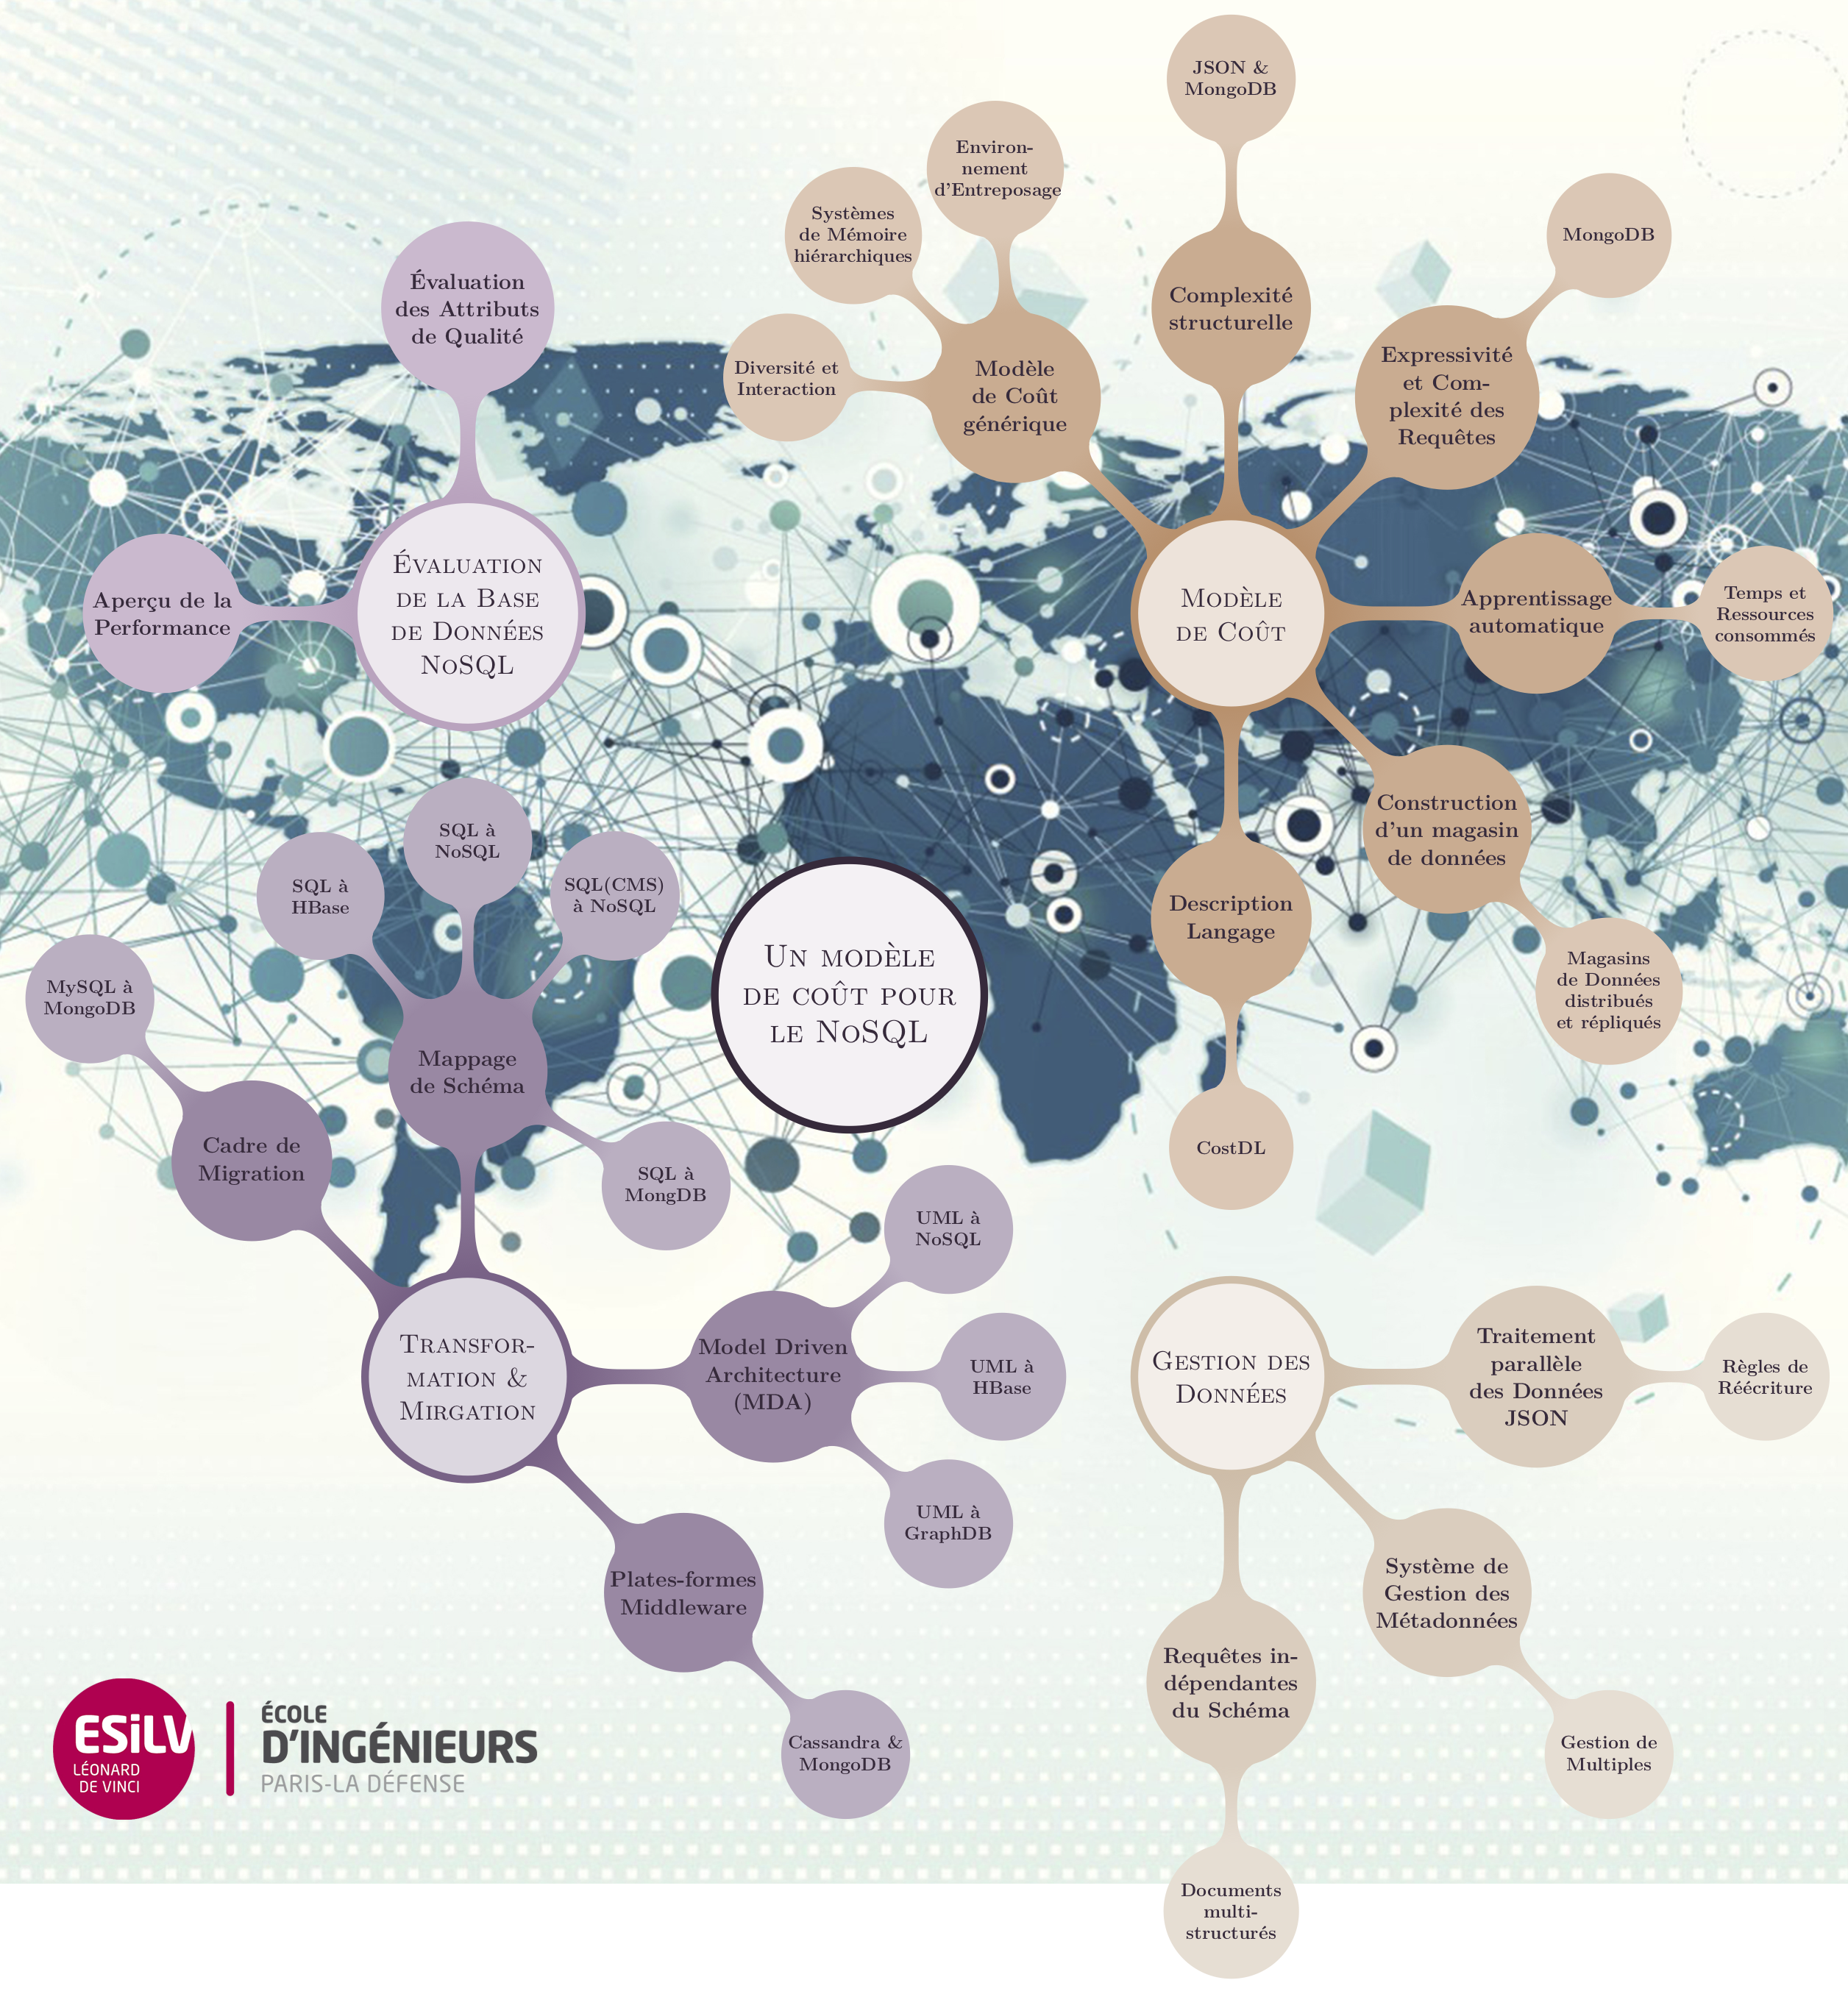
\includegraphics[height = 6.5cm]{images/mindmap.png}
\end{frame}

\section{Hypothèse}
% Page_8
\begin{frame}
\frametitle{Sommaire}
\tableofcontents[currentsection]
\end{frame}


\subsection{Normalisation et Dénormalisation}
% Page_9
\begin{frame}[fragile]
	\frametitle{Normalisation}
	\begin{block}{Normalisation}
		\begin{itemize}
			\item[•] Dans une base de données relationnelle, une forme normale désigne un type de relation particulier entre les entités.
			\item[•] Le but essentiel de la normalisation est d'éviter les anomalies transactionnelles pouvant découler d'une mauvaise modélisation des données et ainsi éviter un certain nombre de problèmes potentiels tels que les anomalies de lecture, les anomalies d'écriture, la redondance des données et la contre-performance.
		\end{itemize}
	\end{block}
\end{frame}

% Page_10
\begin{frame}[fragile]
	\frametitle{Dénormalisation}
	\begin{block}{Dénormalisation}
	\begin{itemize}
			\item[•] La dénormalisation peut être définie comme la copie des mêmes données dans plusieurs documents ou tables afin de simplifier / optimiser le traitement des requêtes ou d’adapter les données de l’utilisateur à un modèle de données particulier. Elle  permet de stocker des données dans une structure adaptée pour simplifier le traitement des requêtes. L’objectif pour les systèmes NoSQL est de proposer un schéma de stockage permettant d’éviter l’utilisation des jointures pour lesquelles les systèmes NoSQL sont peu adaptés en raison de l’architecture distribuée sous-jacente.
			\item[•]Systèmes applicables :  dépôts  clé-valeur, bases de données document, bases de données colonnes.
	\end{itemize}
	\end{block}
\end{frame}

% Page_11
\subsection{Objectif de recherche}
\begin{frame}{Objectif de recherche}
	\begin{itemize}
		\item[•] Comparer la durée pendant laquelle les bases de données (normalisées ou dénormalisées) de différentes tailles répondent aux quatre principaux types de commandes(CRUD), c'est-à-dire comparer leurs modèles de coût sur temps.
		\item[•] À l’avenir, sur la base des résultats obtenus, comparez les théories existantes et découvrez les lois mathématiques.
	\end{itemize}
\end{frame}

% Page_12
\section{Démarche Expérimentale}
\begin{frame}
\frametitle{Sommaire}
\tableofcontents[currentsection]
\end{frame}

% Page_13
\subsection{Modélisation}
\begin{frame}{Schéma}
		\includegraphics[height = 2cm]{images/TPCC.pdf}
\end{frame}

% Page_14
\begin{frame}{Modélisation}
		\includegraphics[height = 6.5cm]{images/modelisation.png}
\end{frame}

% Page_15
\subsection{Quatre requêtes de CRUD}
\begin{frame}{Quatre requêtes de CRUD}
	\begin{itemize}
		\item[•] La requête C, créer une nouvelle commande avec 10 articles différents
		\item[•] La requête R, chercher aléatoirement l’information d’un client par son nom et prénom en montrant l’id de la plus nouvelle commande.
		\item[•] La requête U, modifier le temps de livraison des dix articles les plus anciens qui ne sont pas encore délivrés
		\item[•] La requête D, supprimer aléatoirement d’une commande pas encore livrée.
	\end{itemize}
\end{frame}

% Page_16
\section{Résultats et conclusion}
\begin{frame}
\frametitle{Sommaire}
\tableofcontents[currentsection]
\end{frame}

% Page_17
\begin{frame}{Résultats }
		\includegraphics[height = 6.5cm]{images/image_1.png}
\end{frame}

% Page_18
\begin{frame}{Résultats}
		\includegraphics[height = 6.5cm]{images/image_2.png}
\end{frame}

% Page_19
\begin{frame}{Conclusion}
À cause de temps limité, la recherche actuelle sur le modèle de coût de la base de données NoSQL est encore au stade initial de la modélisation.  Au cours du processus, j'ai rencontré de nombreux problèmes, tels que le temps de fusion de la base de données est trop long ou le langage de requête n'est pas assez précis. Une fois la modélisation actuelle mise au point, il est nécessaire de répéter les pratiques pour obtenir un résultat de test plus crédible.Quant à savoir si nous pouvons enfin trouver une loi crédible, vous devez la tester tout le temps.
\end{frame}

% Page_20
\begin{frame}{Perspective}
Pour un sujet axé sur la recherche, sa tâche ne doit pas se limiter à des tests, mais en être déduite. Par conséquent, pour ce sujet, lorsque les résultats des tests de tous les cent entrepôts de données sont établis, il est naturel de combiner la littérature scientifique pour en déduire des lois et même des formules de données. Les facteurs affectant cette formule peuvent être nombreux, tels que les performances de la machine ou la complexité de la structure.
\end{frame}

\end{document}